\appendix
\addcontentsline{toc}{chapter}{Appendices}
\renewcommand\thefigure{\thesection.\arabic{figure}}

\chapter*{Appendices}
\renewcommand{\thesection}{\Alph{section}}

\section{Software user guide}
The code is organized in several modules:
\begin{itemize}
	\itemsep-0.3em 
	\item \textbf{root}, contains files:
	\begin{itemize}
		\itemsep-0.3em 
		\item \textit{play.py} starts the program in play mode. 
		\item \textit{train.py} starts the algorithm in training mode.
		\item \textit{controller.py} handles playing the game, when the program is in play mode, between two opponents. Conceptually it belongs in module \textit{hex}, but placed here because of how Python handles disk file lookup.
	\end{itemize}
	\item \textbf{nnsc}, with the following files:
	\begin{itemize}
		\itemsep-0.3em 
		\item \textit{nnsc.py}, contains the runnable algorithm, both the when it is in training mode and in play mode.
		\item \textit{config.py}, contains a class of the same name, that holds all the important tweakable parameters for the algorithm. 
		\item \textit{network.py}, contains the neural network.
		\item \textit{gamestorage.py}, contains a class that keeps, in accordance with a config value, the most recent self-played games in memory, for use in training the network. It is also tasked with creating data batches of images of said games.
		\item \textit{savefile.py}, contains a self-titled class, that is able to save all important objects to disk, such that the algorithm can be stopped at a certain time, and restarted later, with the same network, gamestorage, config, etc.
	\end{itemize}
	\item \textbf{hex}, with the following files:
	\begin{itemize}
		\itemsep-0.3em 
		\item \textit{gui.py}, allows for a visual and, in the case of a human player, interactive representation of a game.
		\item \textit{game.py}, contains all the game specific implementation for the game of Hex.
	\end{itemize}
	\item \textbf{ais}, contains \textit{mcts.py}, which is a simple purely UCT based agent, and \textit{random.py}, which is an agent that takes random actions. Both of these have been used for testing that the learned agents are actually increasing their ability to play the game well. 
\end{itemize}

When play.py is run it requires 5 or 6 ordered arguments. The 2 first are which agents that should play, the 3rd is the board size, the 4th is the amount of games to play, and the 5th is an optional parameter \textit{vis}, which sets the game to be played with a visual interface. Running play from a terminal could look like this:

\begin{displayquote}
{\normalfont\ttfamily python play.py nn!az mcts!2000 7 2 vis}
\end{displayquote}

Several, unordered, optional arguments, separated by spaces, can be given to train.py. Except for the paramaters \textit{save=<filename>} and \textit{load=<filename>}, if a specific argument setting is not provided, a default value will be used, in creating a config object. Running train.py from a terminal can be as simple as this:

\begin{displayquote}
{\normalfont\ttfamily python train.py save=new-test size=13}
\end{displayquote}

The parameters used for the config object, when using train.py, are:
\begin{itemize}
	\itemsep-0.3em 
	\item \textit{size=<value>}. Sets the board shape as $size\times size$. Default value is 9.
	\item \textit{sims=<value>}. Sets the number of simulations the MCTS part of the algorithm uses. Default value is 200.
	\item \textit{blocks=<value>}. Set the number of residual blocks that are used in the neural network. Default value is 19.
	\item \textit{filters=<value>}. Sets the number of channels in the convolutional layers  of the residual blocks, such that the shape of input and output will be $batch\_size \times filtes \times size \ size$. Default value is 256.
	\item \textit{actors=<value>}. Sets the amount of self-played games to be in played in batch between training the network. Default value is 50.
	\item \textit{epochs=<value>}. Sets the number of training iterations to be performed between each batch of self-playing. Default value is 10.
	\item \textit{window=<value>}. Sets the amount of most recet self-played games to be saved in gamestorage. Default value is 1000.
	\item \textit{batch=<value>}. Sets the size of the image dataset used for the individual training iterations. Default value is 512.
	\item \textit{singleprecision}. Sets the model to be using single-precision, both during training and self-playing. Default value is that mixed-precision is used. 
	\item \textit{type=<type>}. If none are set the algorithm will work similar to what is shown in figure \ref{fig-targets-az}, and use the original residual block design, as shown in figure \ref{fig-res-block}. The \textit{<type>} can be one of the following:
	\begin{itemize}
		\itemsep-0.3em
		\item \textit{u}. Sets the MCTS part of the algorithm to use the utility function for terminal states. See figure \ref{fig-targets-util}.
		\item \textit{q}. Sets the algorithm to use average mean value of root states as training value target, in accordance with figure \ref{fig-targets-q}.
		\item \textit{fpa}. Sets the model to follow both \textit{q} and use full pre-activation block design in the neural network, as seen in figure \ref{fig-fpa-block}.
	\end{itemize}
\end{itemize}

It is recommended to run the program from a console user interface that has extensive support for ANSI, since the program uses prints that manipulate the console output through escape sequences.

The following packages are also needed:
\begin{ttfamily}

pytorch (a GPU supporting CUDA is necessary)\\
torchvision\\
pillow\\
pickle\\
tk\\
matplotlib\\
numpy\\
numba\\
\end{ttfamily}
\clearpage
\section{Selected matches against Hexy}
Eight games are included here, with history provided by labels on each piece, indicating when in the sequence of play it was placed.

All games feature Hexy on expert settings, a game as first, and one as second, against: H1 with 1200 training iterations; H2 with 1,200 training iterations; H2 with 2400 training iterations; and the baseline MCTS with 10,000 simulations.

This selection has been made with the attitude that it is most interesting to see how the best performing agents are playing, and in regards to MCTS, get a perspective of what type of decisions it makes.

Hexy wins all of them except one, figure \ref{fig-h2-2400-hexy}. This against H2 with 2,400 training iterations, where Hexy is the second player (dark).

\begin{figure}[ht]
	\centering
	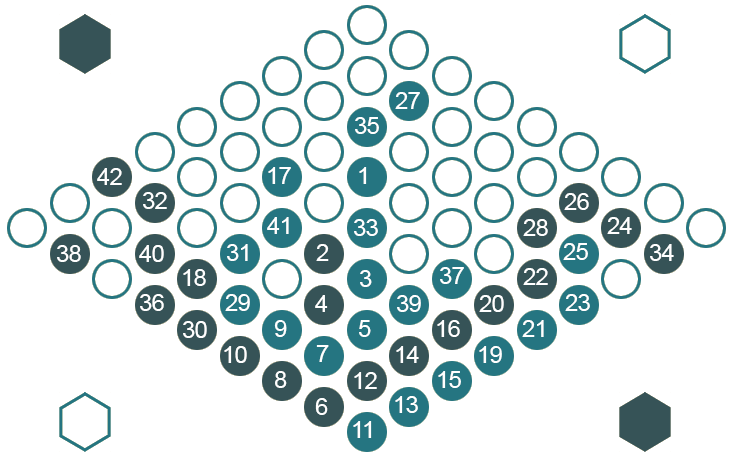
\includegraphics[width=.75\textwidth]{graphics/games/h1-1200-hexy.png}
	\caption{H1 1200 (light) vs Hexy (dark). Winner: Hexy}
	\label{fig-h1-1200-hexy}
\end{figure}
\vspace{1cm}

\begin{figure}[ht]
	\centering
	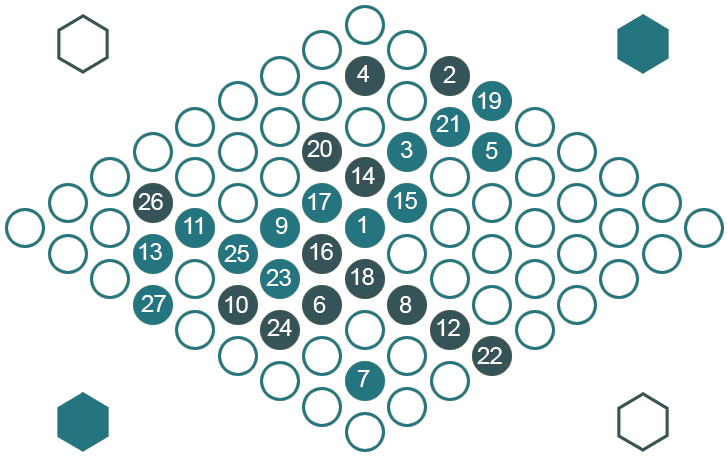
\includegraphics[width=.75\textwidth]{graphics/games/hexy-h1-1200.png}
	\caption{Hexy (light) vs H1 1200 (dark). Winner: Hexy}
	\label{fig-hexy-h1-1200}
\end{figure}
\vspace{1cm}

\begin{figure}[ht]
	\centering
	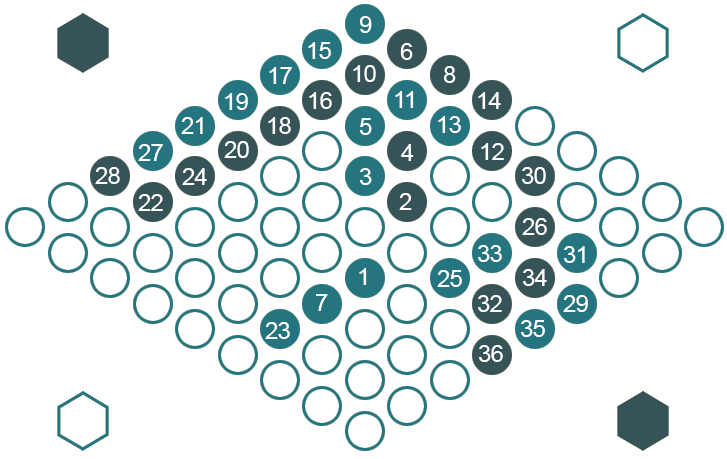
\includegraphics[width=.75\textwidth]{graphics/games/h2-1200-hexy.png}
	\caption{H2 1200 (light) vs Hexy (dark). Winner: Hexy}
	\label{fig-h2-1200-hexy}
\end{figure}
\vspace{1cm}

\begin{figure}[ht]
	\centering
	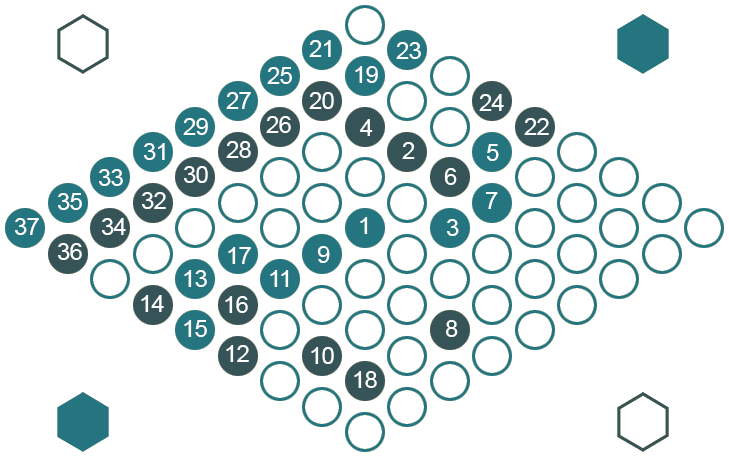
\includegraphics[width=.75\textwidth]{graphics/games/hexy-h2-1200.png}
	\caption{Hexy (light) vs H2 1200 (dark). Winner: Hexy}
	\label{fig-hexy-h2-1200}
\end{figure}
\vspace{1cm}

\begin{figure}[ht]
	\centering
	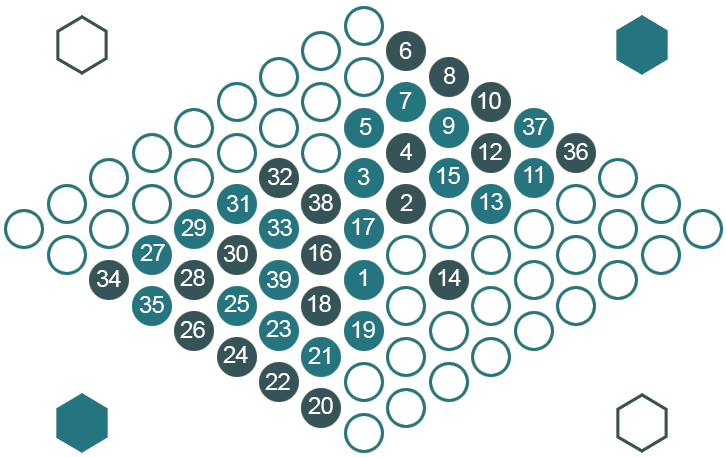
\includegraphics[width=.75\textwidth]{graphics/games/h2-2400-hexy.png}
	\caption{H2 2400 (light) vs Hexy (dark). Winner: H2 2400}
	\label{fig-h2-2400-hexy}
\end{figure}
\vspace{1cm}

\begin{figure}[ht]
	\centering
	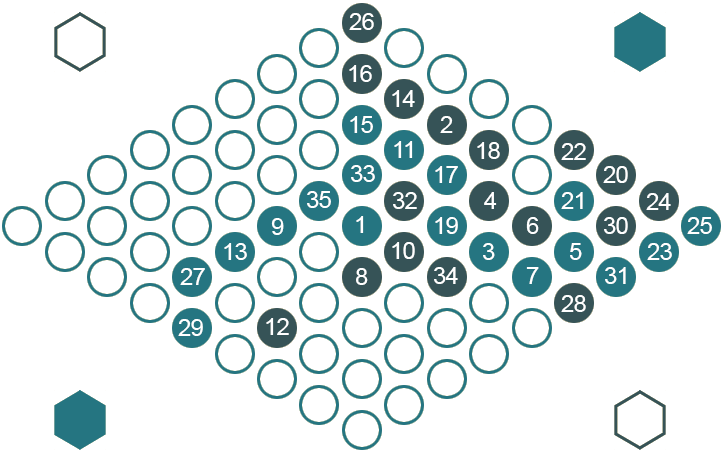
\includegraphics[width=.75\textwidth]{graphics/games/hexy-h2-2400.png}
	\caption{Hexy (light) vs H2 2400 (dark). Winner: Hexy}
	\label{fig-hexy-h2-2400}
\end{figure}
\vspace{1cm}

\begin{figure}[ht]
	\centering
	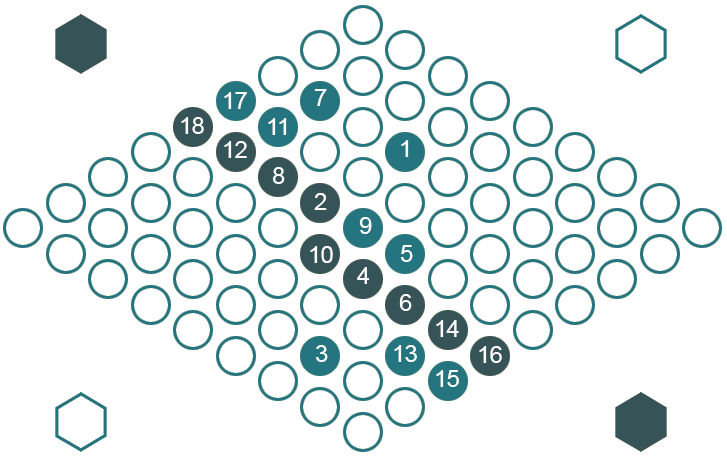
\includegraphics[width=.75\textwidth]{graphics/games/mcts-hexy.png}
	\caption{baseline MCTS (light) vs Hexy (dark). Winner: Hexy}
	\label{fig-mcts-hexy}
\end{figure}
\vspace{1cm}
\begin{figure}[ht]
	\centering
	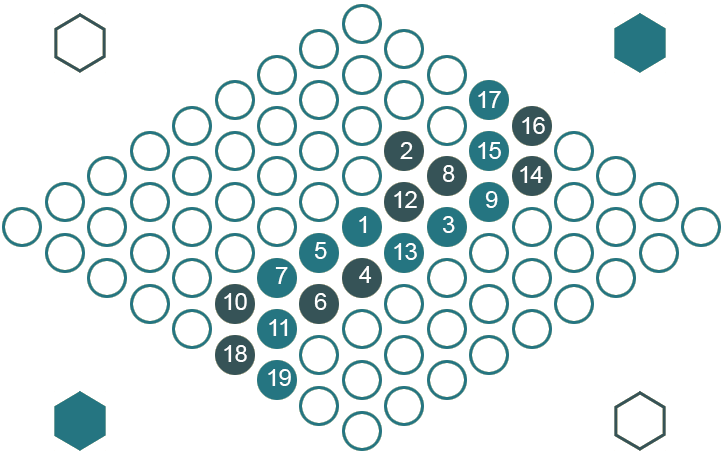
\includegraphics[width=.75\textwidth]{graphics/games/hexy-mcts.png}
	\caption{Hexy (light) vs baseline MCTS (dark). Winner: Hexy}
	\label{fig-hexy-mcts}
\end{figure}


\clearpage
\section{Bayesian Elo estimation tables}
Below is the output of running the tool \cite{Coulom} from \citeauthor{Coulom}, with the game results found in Appendix D.

\begin{table}[ht]
\small
\centering
\begin{tabular}{ c c c c c c c c c}
Rank & Name                   & Elo &   +  &  - &games &score &oppo. &draws\\
\hline
   1& Hexy (expert)          & 888&  343&  212  &  30 & 100\% &  -59 &   0\%\\
\hline
   2& H2 1200                & 659&  183&  150  &  38 &  89\% &   30 &   0\%\\
\hline
   3& H1 1200                & 644&  179&  143  &  38 &  89\% &   31 &   0\%\\
\hline
   4& H1 1000                & 478&  145&  132  &  38 &  79\% &   40 &   0\%\\
\hline
   5& baseline MCTS (10000)  & 307&   79&   76  & 142 &  75\% &  -72 &   0\%\\
\hline
   6& H2 1000                & 225&  129&  130  &  38 &  61\% &   53 &   0\%\\
\hline
   7& H1 800                 & 190&  131&  133  &  38 &  58\% &   55 &   0\%\\
\hline
   8& H2 800                 & -19&  131&  140  &  38 &  42\% &   66 &   0\%\\
\hline
   9& H1 600                 & -56&  132&  141  &  38 &  39\% &   68 &   0\%\\
\hline
  10& H2 600                 &-177&  138&  146  &  38 &  32\% &   74 &   0\%\\
\hline
  11& H2 400                 &-263&  143&  150  &  38 &  26\% &   79 &   0\%\\
\hline
  12& H1 400                 &-400&  150&  164  &  38 &  18\% &   86 &   0\%\\
\hline
  13& H1 200                 &-504&  158&  178  &  38 &  13\% &   91 &   0\%\\
\hline
  14& H2 200                 &-505&  161&  182  &  38 &  13\% &   91 &   0\%\\
\hline
  15& H1 0                   &-620&  167&  203  &  38 &   8\% &   97 &   0\%\\
\hline
  16& H2 0                   &-848&  199&  339  &  38 &   0\% &  109 &   0\%\\
\hline
\end{tabular}
\end{table}

Adding the two games between Hexy and H2, with 2,400 training iterations, gives the following table:

\begin{table}[ht]
\small
\centering
\begin{tabular}{ c c c c c c c c c}

Rank &Name&                    Elo  &  +  &  - &games &score &oppo. &draws \\
\hline
   1& Hexy (expert)         &  843&  229&  181  &  32 &  97\%  & -53 &   0\%\\
\hline
   2& H2 2400               &  843&  335&  342  &   2 &  50\%  & 843 &   0\%\\
\hline
   3& H2 1200               &  607&  184&  151  &  38 &  89\%  & -23 &   0\%\\
\hline
   4& H1 1200               &  593&  180&  144  &  38 &  89\%  & -22  &  0\%\\
\hline
   5& H1 1000               &  426&  146&  132  &  38 &  79\%  & -13  &  0\%\\
\hline
   6& baseline MCTS (10000) &  254&   79&   76  & 142 &  75\%  &-125  &  0\%\\
\hline
   7& H2 1000               &  172&  130&  131  &  38 &  61\%  &   0  &  0\%\\
\hline
   8& H1 800                &  137&  132&  134  &  38 &  58\%  &   2  &  0\%\\
\hline
   9& H2 800                &  -73&  132&  141  &  38 &  42\%  &  13  &  0\%\\
\hline
  10& H1 600                & -109&  132&  142  &  38 &  39\%  &  15  &  0\%\\
\hline
  11& H2 600                & -230&  139&  147  &  38 &  32\%  &  21  &  0\%\\
\hline
  12& H2 400                & -317&  143&  151  &  38 &  26\%  &  26  &  0\%\\
\hline
  13& H1 400                & -453&  151&  165  &  38 &  18\%  &  33  &  0\%\\
\hline
  14& H1 200                & -558&  158&  179  &  38 &  13\%  &  39  &  0\%\\
\hline
  15& H2 200                & -559&  161&  183  &  38 &  13\%  &  39  &  0\%\\
\hline
  16& H1 0                  & -675&  168&  204  &  38 &   8\%  &  45  &  0\%\\
\hline
  17& H2 0                  & -903&  200&  333  &  38 &   0\%  &  57  &  0\%\\
  \hline
\end{tabular}
\end{table}

\clearpage
\section{Game results used in Elo estimation}
All results are in Portable Game Notation (PGN), such that it can be parsed by the freeware tool\cite{Coulom} used to estimate Bayesian Elo ratings.

{\ttfamily
[Date "2019-05-13 01:40:16.182317"]
[White "H1 0"]
[Black "H1 1000"]
[Result "0-1"]
.

[Date "2019-05-13 01:35:32.181218"]
[White "H1 0"]
[Black "H1 1200"]
[Result "0-1"]
.

[Date "2019-05-13 02:00:59.765688"]
[White "H1 0"]
[Black "H1 200"]
[Result "0-1"]
.

[Date "2019-05-13 01:52:47.839595"]
[White "H1 0"]
[Black "H1 400"]
[Result "0-1"]
.

[Date "2019-05-13 01:47:33.025522"]
[White "H1 0"]
[Black "H1 600"]
[Result "0-1"]
.

[Date "2019-05-13 01:44:25.662522"]
[White "H1 0"]
[Black "H1 800"]
[Result "0-1"]
.

[Date "2019-05-13 11:18:02.053649"]
[White "H1 0"]
[Black "H2 0"]
[Result "1-0"]
.

[Date "2019-05-13 12:02:12.021380"]
[White "H1 0"]
[Black "H2 1000"]
[Result "0-1"]
.

[Date "2019-05-13 12:05:27.367748"]
[White "H1 0"]
[Black "H2 1200"]
[Result "0-1"]
.

[Date "2019-05-13 11:34:25.461840"]
[White "H1 0"]
[Black "H2 200"]
[Result "1-0"]
.

[Date "2019-05-13 11:40:59.225788"]
[White "H1 0"]
[Black "H2 400"]
[Result "0-1"]
.

[Date "2019-05-13 11:51:38.370201"]
[White "H1 0"]
[Black "H2 600"]
[Result "0-1"]
.

[Date "2019-05-13 11:56:12.637533"]
[White "H1 0"]
[Black "H2 800"]
[Result "0-1"]
.

[Date "2019-05-14 11:19:22.907988"]
[White "H1 0"]
[Black "Hexy (expert)"]
[Result "0-1"]
.

[Date "2019-05-10 20:18:40.588810"]
[White "H1 0"]
[Black "baseline MCTS (10000)"]
[Result "0-1"]
.

[Date "2019-05-10 20:18:40.604416"]
[White "H1 0"]
[Black "baseline MCTS (10000)"]
[Result "0-1"]
.

[Date "2019-05-10 20:18:57.666956"]
[White "H1 0"]
[Black "baseline MCTS (10000)"]
[Result "0-1"]
.

[Date "2019-05-10 20:19:09.853848"]
[White "H1 0"]
[Black "baseline MCTS (10000)"]
[Result "0-1"]
.

[Date "2019-05-10 20:19:17.010675"]
[White "H1 0"]
[Black "baseline MCTS (10000)"]
[Result "0-1"]
.

[Date "2019-05-13 01:42:24.579275"]
[White "H1 1000"]
[Black "H1 0"]
[Result "1-0"]
.

[Date "2019-05-13 03:17:13.807486"]
[White "H1 1000"]
[Black "H1 1200"]
[Result "0-1"]
.

[Date "2019-05-13 02:33:37.487876"]
[White "H1 1000"]
[Black "H1 200"]
[Result "1-0"]
.

[Date "2019-05-13 02:52:15.775194"]
[White "H1 1000"]
[Black "H1 400"]
[Result "1-0"]
.

[Date "2019-05-13 03:04:44.312286"]
[White "H1 1000"]
[Black "H1 600"]
[Result "1-0"]
.

[Date "2019-05-13 03:11:03.540830"]
[White "H1 1000"]
[Black "H1 800"]
[Result "1-0"]
.

[Date "2019-05-13 15:49:42.963906"]
[White "H1 1000"]
[Black "H2 0"]
[Result "1-0"]
.

[Date "2019-05-13 16:42:20.192982"]
[White "H1 1000"]
[Black "H2 1000"]
[Result "1-0"]
.

[Date "2019-05-13 16:49:58.140211"]
[White "H1 1000"]
[Black "H2 1200"]
[Result "0-1"]
.

[Date "2019-05-13 15:55:58.736639"]
[White "H1 1000"]
[Black "H2 200"]
[Result "1-0"]
.

[Date "2019-05-13 15:58:44.299319"]
[White "H1 1000"]
[Black "H2 400"]
[Result "1-0"]
.

[Date "2019-05-13 16:02:07.821846"]
[White "H1 1000"]
[Black "H2 600"]
[Result "1-0"]
.

[Date "2019-05-13 16:16:59.550529"]
[White "H1 1000"]
[Black "H2 800"]
[Result "1-0"]
.

[Date "2019-05-14 10:44:23.917748"]
[White "H1 1000"]
[Black "Hexy (expert)"]
[Result "0-1"]
.

[Date "2019-05-10 15:45:05.057384"]
[White "H1 1000"]
[Black "baseline MCTS (10000)"]
[Result "1-0"]
.

[Date "2019-05-10 15:45:05.057384"]
[White "H1 1000"]
[Black "baseline MCTS (10000)"]
[Result "1-0"]
.

[Date "2019-05-10 15:45:05.073006"]
[White "H1 1000"]
[Black "baseline MCTS (10000)"]
[Result "1-0"]
.

[Date "2019-05-10 15:45:05.073006"]
[White "H1 1000"]
[Black "baseline MCTS (10000)"]
[Result "1-0"]
.

[Date "2019-05-10 15:46:34.760707"]
[White "H1 1000"]
[Black "baseline MCTS (10000)"]
[Result "0-1"]
.

[Date "2019-05-13 01:36:53.984096"]
[White "H1 1200"]
[Black "H1 0"]
[Result "1-0"]
.

[Date "2019-05-13 03:18:41.791167"]
[White "H1 1200"]
[Black "H1 1000"]
[Result "1-0"]
.

[Date "2019-05-13 02:37:55.616850"]
[White "H1 1200"]
[Black "H1 200"]
[Result "1-0"]
.

[Date "2019-05-13 02:56:11.139068"]
[White "H1 1200"]
[Black "H1 400"]
[Result "1-0"]
.

[Date "2019-05-13 03:07:47.149950"]
[White "H1 1200"]
[Black "H1 600"]
[Result "1-0"]
.

[Date "2019-05-13 03:14:37.821696"]
[White "H1 1200"]
[Black "H1 800"]
[Result "1-0"]
.

[Date "2019-05-13 17:01:46.893910"]
[White "H1 1200"]
[Black "H2 0"]
[Result "1-0"]
.

[Date "2019-05-13 17:24:19.784844"]
[White "H1 1200"]
[Black "H2 1000"]
[Result "1-0"]
.

[Date "2019-05-13 17:28:09.587846"]
[White "H1 1200"]
[Black "H2 1200"]
[Result "0-1"]
.

[Date "2019-05-13 17:08:31.133450"]
[White "H1 1200"]
[Black "H2 200"]
[Result "1-0"]
.

[Date "2019-05-13 17:11:14.429410"]
[White "H1 1200"]
[Black "H2 400"]
[Result "1-0"]
.

[Date "2019-05-13 17:18:33.714111"]
[White "H1 1200"]
[Black "H2 600"]
[Result "1-0"]
.

[Date "2019-05-13 17:21:10.588056"]
[White "H1 1200"]
[Black "H2 800"]
[Result "1-0"]
.

[Date "2019-05-13 20:32:04.594733"]
[White "H1 1200"]
[Black "Hexy (expert)"]
[Result "0-1"]
.

[Date "2019-05-10 14:42:40.651265"]
[White "H1 1200"]
[Black "baseline MCTS (10000)"]
[Result "1-0"]
.

[Date "2019-05-10 14:42:40.651265"]
[White "H1 1200"]
[Black "baseline MCTS (10000)"]
[Result "1-0"]
.

[Date "2019-05-10 14:42:40.651265"]
[White "H1 1200"]
[Black "baseline MCTS (10000)"]
[Result "1-0"]
.

[Date "2019-05-10 14:42:40.651265"]
[White "H1 1200"]
[Black "baseline MCTS (10000)"]
[Result "1-0"]
.

[Date "2019-05-10 14:42:40.651265"]
[White "H1 1200"]
[Black "baseline MCTS (10000)"]
[Result "1-0"]
.

[Date "2019-05-13 02:05:37.641503"]
[White "H1 200"]
[Black "H1 0"]
[Result "1-0"]
.

[Date "2019-05-13 02:31:51.412135"]
[White "H1 200"]
[Black "H1 1000"]
[Result "0-1"]
.

[Date "2019-05-13 02:36:01.576174"]
[White "H1 200"]
[Black "H1 1200"]
[Result "0-1"]
.

[Date "2019-05-13 02:13:50.637708"]
[White "H1 200"]
[Black "H1 400"]
[Result "0-1"]
.

[Date "2019-05-13 02:21:44.896859"]
[White "H1 200"]
[Black "H1 600"]
[Result "0-1"]
.

[Date "2019-05-13 02:25:54.164797"]
[White "H1 200"]
[Black "H1 800"]
[Result "0-1"]
.

[Date "2019-05-13 12:12:56.530194"]
[White "H1 200"]
[Black "H2 0"]
[Result "1-0"]
.

[Date "2019-05-13 13:01:21.668023"]
[White "H1 200"]
[Black "H2 1000"]
[Result "0-1"]
.

[Date "2019-05-13 13:04:06.247964"]
[White "H1 200"]
[Black "H2 1200"]
[Result "0-1"]
.

[Date "2019-05-13 12:24:14.961188"]
[White "H1 200"]
[Black "H2 200"]
[Result "0-1"]
.

[Date "2019-05-13 12:29:14.146946"]
[White "H1 200"]
[Black "H2 400"]
[Result "0-1"]
.

[Date "2019-05-13 12:43:49.905060"]
[White "H1 200"]
[Black "H2 600"]
[Result "0-1"]
.

[Date "2019-05-13 12:49:26.232096"]
[White "H1 200"]
[Black "H2 800"]
[Result "0-1"]
.

[Date "2019-05-14 11:09:45.249564"]
[White "H1 200"]
[Black "Hexy (expert)"]
[Result "0-1"]
.

[Date "2019-05-10 19:24:27.332784"]
[White "H1 200"]
[Black "baseline MCTS (10000)"]
[Result "0-1"]
.

[Date "2019-05-10 19:24:48.102509"]
[White "H1 200"]
[Black "baseline MCTS (10000)"]
[Result "0-1"]
.

[Date "2019-05-10 19:24:48.102509"]
[White "H1 200"]
[Black "baseline MCTS (10000)"]
[Result "0-1"]
.

[Date "2019-05-10 19:25:10.354975"]
[White "H1 200"]
[Black "baseline MCTS (10000)"]
[Result "0-1"]
.

[Date "2019-05-10 19:25:17.712629"]
[White "H1 200"]
[Black "baseline MCTS (10000)"]
[Result "0-1"]
.

[Date "2019-05-13 01:54:45.391561"]
[White "H1 400"]
[Black "H1 0"]
[Result "1-0"]
.

[Date "2019-05-13 02:50:40.457760"]
[White "H1 400"]
[Black "H1 1000"]
[Result "0-1"]
.

[Date "2019-05-13 02:54:21.634212"]
[White "H1 400"]
[Black "H1 1200"]
[Result "0-1"]
.

[Date "2019-05-13 02:16:21.902774"]
[White "H1 400"]
[Black "H1 200"]
[Result "1-0"]
.

[Date "2019-05-13 02:40:32.028441"]
[White "H1 400"]
[Black "H1 600"]
[Result "0-1"]
.

[Date "2019-05-13 02:45:31.974640"]
[White "H1 400"]
[Black "H1 800"]
[Result "0-1"]
.

[Date "2019-05-13 13:09:55.067215"]
[White "H1 400"]
[Black "H2 0"]
[Result "1-0"]
.

[Date "2019-05-13 13:55:15.115340"]
[White "H1 400"]
[Black "H2 1000"]
[Result "0-1"]
.

[Date "2019-05-13 13:58:37.408960"]
[White "H1 400"]
[Black "H2 1200"]
[Result "0-1"]
.

[Date "2019-05-13 13:17:16.425484"]
[White "H1 400"]
[Black "H2 200"]
[Result "0-1"]
.

[Date "2019-05-13 13:33:07.603515"]
[White "H1 400"]
[Black "H2 400"]
[Result "0-1"]
.

[Date "2019-05-13 13:42:11.015936"]
[White "H1 400"]
[Black "H2 600"]
[Result "0-1"]
.

[Date "2019-05-13 13:51:28.645154"]
[White "H1 400"]
[Black "H2 800"]
[Result "0-1"]
.

[Date "2019-05-14 11:00:59.853297"]
[White "H1 400"]
[Black "Hexy (expert)"]
[Result "0-1"]
.

[Date "2019-05-10 18:28:25.855082"]
[White "H1 400"]
[Black "baseline MCTS (10000)"]
[Result "0-1"]
.

[Date "2019-05-10 18:28:25.855082"]
[White "H1 400"]
[Black "baseline MCTS (10000)"]
[Result "0-1"]
.

[Date "2019-05-10 18:28:59.447215"]
[White "H1 400"]
[Black "baseline MCTS (10000)"]
[Result "0-1"]
.

[Date "2019-05-10 18:29:19.134569"]
[White "H1 400"]
[Black "baseline MCTS (10000)"]
[Result "0-1"]
.

[Date "2019-05-10 18:29:25.525917"]
[White "H1 400"]
[Black "baseline MCTS (10000)"]
[Result "0-1"]
.

[Date "2019-05-13 01:49:06.149342"]
[White "H1 600"]
[Black "H1 0"]
[Result "1-0"]
.

[Date "2019-05-13 03:03:02.597588"]
[White "H1 600"]
[Black "H1 1000"]
[Result "0-1"]
.

[Date "2019-05-13 03:06:35.548619"]
[White "H1 600"]
[Black "H1 1200"]
[Result "0-1"]
.

[Date "2019-05-13 02:23:29.382711"]
[White "H1 600"]
[Black "H1 200"]
[Result "1-0"]
.

[Date "2019-05-13 02:42:29.981300"]
[White "H1 600"]
[Black "H1 400"]
[Result "1-0"]
.

[Date "2019-05-13 02:58:51.619405"]
[White "H1 600"]
[Black "H1 800"]
[Result "0-1"]
.

[Date "2019-05-13 14:01:56.357969"]
[White "H1 600"]
[Black "H2 0"]
[Result "1-0"]
.

[Date "2019-05-13 15:10:06.162725"]
[White "H1 600"]
[Black "H2 1000"]
[Result "0-1"]
.

[Date "2019-05-13 15:16:27.884458"]
[White "H1 600"]
[Black "H2 1200"]
[Result "0-1"]
.

[Date "2019-05-13 14:05:49.103323"]
[White "H1 600"]
[Black "H2 200"]
[Result "1-0"]
.

[Date "2019-05-13 14:26:46.469500"]
[White "H1 600"]
[Black "H2 400"]
[Result "1-0"]
.

[Date "2019-05-13 14:32:29.221552"]
[White "H1 600"]
[Black "H2 600"]
[Result "1-0"]
.

[Date "2019-05-13 14:38:34.369554"]
[White "H1 600"]
[Black "H2 800"]
[Result "0-1"]
.

[Date "2019-05-14 10:55:25.661114"]
[White "H1 600"]
[Black "Hexy (expert)"]
[Result "0-1"]
.

[Date "2019-05-10 17:34:28.558310"]
[White "H1 600"]
[Black "baseline MCTS (10000)"]
[Result "0-1"]
.

[Date "2019-05-10 17:34:28.558310"]
[White "H1 600"]
[Black "baseline MCTS (10000)"]
[Result "0-1"]
.

[Date "2019-05-10 17:34:28.558310"]
[White "H1 600"]
[Black "baseline MCTS (10000)"]
[Result "0-1"]
.

[Date "2019-05-10 17:34:40.604243"]
[White "H1 600"]
[Black "baseline MCTS (10000)"]
[Result "0-1"]
.

[Date "2019-05-10 17:34:48.214014"]
[White "H1 600"]
[Black "baseline MCTS (10000)"]
[Result "0-1"]
.

[Date "2019-05-13 01:45:46.255690"]
[White "H1 800"]
[Black "H1 0"]
[Result "1-0"]
.

[Date "2019-05-13 03:09:53.813889"]
[White "H1 800"]
[Black "H1 1000"]
[Result "0-1"]
.

[Date "2019-05-13 03:13:13.493125"]
[White "H1 800"]
[Black "H1 1200"]
[Result "0-1"]
.

[Date "2019-05-13 02:27:56.283170"]
[White "H1 800"]
[Black "H1 200"]
[Result "1-0"]
.

[Date "2019-05-13 02:47:26.097647"]
[White "H1 800"]
[Black "H1 400"]
[Result "1-0"]
.

[Date "2019-05-13 03:00:38.215981"]
[White "H1 800"]
[Black "H1 600"]
[Result "1-0"]
.

[Date "2019-05-13 15:19:10.024845"]
[White "H1 800"]
[Black "H2 0"]
[Result "1-0"]
.

[Date "2019-05-13 15:37:27.712918"]
[White "H1 800"]
[Black "H2 1000"]
[Result "0-1"]
.

[Date "2019-05-13 15:44:43.571846"]
[White "H1 800"]
[Black "H2 1200"]
[Result "0-1"]
.

[Date "2019-05-13 15:21:56.319896"]
[White "H1 800"]
[Black "H2 200"]
[Result "1-0"]
.

[Date "2019-05-13 15:25:15.466545"]
[White "H1 800"]
[Black "H2 400"]
[Result "1-0"]
.

[Date "2019-05-13 15:28:25.947237"]
[White "H1 800"]
[Black "H2 600"]
[Result "1-0"]
.

[Date "2019-05-13 15:31:14.881409"]
[White "H1 800"]
[Black "H2 800"]
[Result "1-0"]
.

[Date "2019-05-14 10:50:55.653867"]
[White "H1 800"]
[Black "Hexy (expert)"]
[Result "0-1"]
.

[Date "2019-05-10 16:38:46.260174"]
[White "H1 800"]
[Black "baseline MCTS (10000)"]
[Result "1-0"]
.

[Date "2019-05-10 16:38:46.260174"]
[White "H1 800"]
[Black "baseline MCTS (10000)"]
[Result "1-0"]
.

[Date "2019-05-10 16:38:46.260174"]
[White "H1 800"]
[Black "baseline MCTS (10000)"]
[Result "1-0"]
.

[Date "2019-05-10 16:38:46.260174"]
[White "H1 800"]
[Black "baseline MCTS (10000)"]
[Result "1-0"]
.

[Date "2019-05-10 16:39:16.806424"]
[White "H1 800"]
[Black "baseline MCTS (10000)"]
[Result "0-1"]
.

[Date "2019-05-13 11:22:49.043012"]
[White "H2 0"]
[Black "H1 0"]
[Result "0-1"]
.

[Date "2019-05-13 15:50:57.945914"]
[White "H2 0"]
[Black "H1 1000"]
[Result "0-1"]
.

[Date "2019-05-13 17:02:56.634249"]
[White "H2 0"]
[Black "H1 1200"]
[Result "0-1"]
.

[Date "2019-05-13 12:16:55.377829"]
[White "H2 0"]
[Black "H1 200"]
[Result "0-1"]
.

[Date "2019-05-13 13:11:45.947415"]
[White "H2 0"]
[Black "H1 400"]
[Result "0-1"]
.

[Date "2019-05-13 14:03:29.041255"]
[White "H2 0"]
[Black "H1 600"]
[Result "0-1"]
.

[Date "2019-05-13 15:20:27.925181"]
[White "H2 0"]
[Black "H1 800"]
[Result "0-1"]
.

[Date "2019-05-13 18:16:00.131347"]
[White "H2 0"]
[Black "H2 1000"]
[Result "0-1"]
.

[Date "2019-05-13 18:23:06.836811"]
[White "H2 0"]
[Black "H2 1200"]
[Result "0-1"]
.

[Date "2019-05-13 17:36:33.805391"]
[White "H2 0"]
[Black "H2 200"]
[Result "0-1"]
.

[Date "2019-05-13 17:57:30.025009"]
[White "H2 0"]
[Black "H2 400"]
[Result "0-1"]
.

[Date "2019-05-13 18:02:50.400062"]
[White "H2 0"]
[Black "H2 600"]
[Result "0-1"]
.

[Date "2019-05-13 18:09:31.757944"]
[White "H2 0"]
[Black "H2 800"]
[Result "0-1"]
.

[Date "2019-05-14 03:55:07.322349"]
[White "H2 0"]
[Black "Hexy (expert)"]
[Result "0-1"]
.

[Date "2019-05-11 12:01:43.497182"]
[White "H2 0"]
[Black "baseline MCTS (10000)"]
[Result "0-1"]
.

[Date "2019-05-11 12:02:27.255355"]
[White "H2 0"]
[Black "baseline MCTS (10000)"]
[Result "0-1"]
.

[Date "2019-05-11 12:02:27.264330"]
[White "H2 0"]
[Black "baseline MCTS (10000)"]
[Result "0-1"]
.

[Date "2019-05-11 12:02:27.270314"]
[White "H2 0"]
[Black "baseline MCTS (10000)"]
[Result "0-1"]
.

[Date "2019-05-11 12:03:57.200339"]
[White "H2 0"]
[Black "baseline MCTS (10000)"]
[Result "0-1"]
.

[Date "2019-05-13 12:03:16.041876"]
[White "H2 1000"]
[Black "H1 0"]
[Result "1-0"]
.

[Date "2019-05-13 16:43:26.649989"]
[White "H2 1000"]
[Black "H1 1000"]
[Result "0-1"]
.

[Date "2019-05-13 17:25:29.698274"]
[White "H2 1000"]
[Black "H1 1200"]
[Result "0-1"]
.

[Date "2019-05-13 13:02:27.358103"]
[White "H2 1000"]
[Black "H1 200"]
[Result "1-0"]
.

[Date "2019-05-13 13:56:27.429037"]
[White "H2 1000"]
[Black "H1 400"]
[Result "1-0"]
.

[Date "2019-05-13 15:11:39.530498"]
[White "H2 1000"]
[Black "H1 600"]
[Result "1-0"]
.

[Date "2019-05-13 15:39:01.619823"]
[White "H2 1000"]
[Black "H1 800"]
[Result "1-0"]
.

[Date "2019-05-13 18:17:12.711501"]
[White "H2 1000"]
[Black "H2 0"]
[Result "1-0"]
.

[Date "2019-05-13 20:52:50.482337"]
[White "H2 1000"]
[Black "H2 1200"]
[Result "0-1"]
.

[Date "2019-05-13 20:04:16.499386"]
[White "H2 1000"]
[Black "H2 200"]
[Result "1-0"]
.

[Date "2019-05-13 20:20:55.376087"]
[White "H2 1000"]
[Black "H2 400"]
[Result "1-0"]
.

[Date "2019-05-13 20:34:38.374534"]
[White "H2 1000"]
[Black "H2 600"]
[Result "1-0"]
.

[Date "2019-05-13 20:46:41.443999"]
[White "H2 1000"]
[Black "H2 800"]
[Result "1-0"]
.

[Date "2019-05-14 03:34:03.560715"]
[White "H2 1000"]
[Black "Hexy (expert)"]
[Result "0-1"]
.

[Date "2019-05-10 21:37:11.119733"]
[White "H2 1000"]
[Black "baseline MCTS (10000)"]
[Result "1-0"]
.

[Date "2019-05-10 21:37:11.119733"]
[White "H2 1000"]
[Black "baseline MCTS (10000)"]
[Result "1-0"]
.

[Date "2019-05-10 21:38:05.167156"]
[White "H2 1000"]
[Black "baseline MCTS (10000)"]
[Result "0-1"]
.

[Date "2019-05-10 21:38:28.776160"]
[White "H2 1000"]
[Black "baseline MCTS (10000)"]
[Result "0-1"]
.

[Date "2019-05-10 21:38:34.933132"]
[White "H2 1000"]
[Black "baseline MCTS (10000)"]
[Result "0-1"]
.

[Date "2019-05-13 12:06:30.271782"]
[White "H2 1200"]
[Black "H1 0"]
[Result "1-0"]
.

[Date "2019-05-13 16:52:19.424215"]
[White "H2 1200"]
[Black "H1 1000"]
[Result "1-0"]
.

[Date "2019-05-13 17:30:08.724156"]
[White "H2 1200"]
[Black "H1 1200"]
[Result "1-0"]
.

[Date "2019-05-13 13:05:12.658036"]
[White "H2 1200"]
[Black "H1 200"]
[Result "1-0"]
.

[Date "2019-05-13 13:59:55.343055"]
[White "H2 1200"]
[Black "H1 400"]
[Result "1-0"]
.

[Date "2019-05-13 15:17:29.655175"]
[White "H2 1200"]
[Black "H1 600"]
[Result "1-0"]
.

[Date "2019-05-13 15:45:47.774608"]
[White "H2 1200"]
[Black "H1 800"]
[Result "1-0"]
.

[Date "2019-05-13 18:24:05.282108"]
[White "H2 1200"]
[Black "H2 0"]
[Result "1-0"]
.

[Date "2019-05-13 20:53:56.549862"]
[White "H2 1200"]
[Black "H2 1000"]
[Result "1-0"]
.

[Date "2019-05-13 20:07:47.940280"]
[White "H2 1200"]
[Black "H2 200"]
[Result "1-0"]
.

[Date "2019-05-13 20:24:11.714057"]
[White "H2 1200"]
[Black "H2 400"]
[Result "1-0"]
.

[Date "2019-05-13 20:40:32.561448"]
[White "H2 1200"]
[Black "H2 600"]
[Result "1-0"]
.

[Date "2019-05-13 20:49:42.504255"]
[White "H2 1200"]
[Black "H2 800"]
[Result "1-0"]
.

[Date "2019-05-13 21:21:12.539584"]
[White "H2 1200"]
[Black "Hexy (expert)"]
[Result "0-1"]
.

[Date "2019-05-10 20:37:15.573231"]
[White "H2 1200"]
[Black "baseline MCTS (10000)"]
[Result "1-0"]
.

[Date "2019-05-10 20:37:15.588859"]
[White "H2 1200"]
[Black "baseline MCTS (10000)"]
[Result "1-0"]
.

[Date "2019-05-10 20:37:15.588859"]
[White "H2 1200"]
[Black "baseline MCTS (10000)"]
[Result "1-0"]
.

[Date "2019-05-10 20:38:27.299880"]
[White "H2 1200"]
[Black "baseline MCTS (10000)"]
[Result "0-1"]
.

[Date "2019-05-10 20:39:17.845539"]
[White "H2 1200"]
[Black "baseline MCTS (10000)"]
[Result "0-1"]
.

[Date "2019-05-13 11:38:08.022169"]
[White "H2 200"]
[Black "H1 0"]
[Result "1-0"]
.

[Date "2019-05-13 15:57:17.242368"]
[White "H2 200"]
[Black "H1 1000"]
[Result "0-1"]
.

[Date "2019-05-13 17:09:42.379815"]
[White "H2 200"]
[Black "H1 1200"]
[Result "0-1"]
.

[Date "2019-05-13 12:26:39.417151"]
[White "H2 200"]
[Black "H1 200"]
[Result "0-1"]
.

[Date "2019-05-13 13:20:14.891179"]
[White "H2 200"]
[Black "H1 400"]
[Result "0-1"]
.

[Date "2019-05-13 14:06:58.723383"]
[White "H2 200"]
[Black "H1 600"]
[Result "0-1"]
.

[Date "2019-05-13 15:23:05.159472"]
[White "H2 200"]
[Black "H1 800"]
[Result "0-1"]
.

[Date "2019-05-13 17:39:06.194345"]
[White "H2 200"]
[Black "H2 0"]
[Result "1-0"]
.

[Date "2019-05-13 20:02:53.799600"]
[White "H2 200"]
[Black "H2 1000"]
[Result "0-1"]
.

[Date "2019-05-13 20:06:23.946481"]
[White "H2 200"]
[Black "H2 1200"]
[Result "0-1"]
.

[Date "2019-05-13 19:37:58.649780"]
[White "H2 200"]
[Black "H2 400"]
[Result "0-1"]
.

[Date "2019-05-13 19:51:43.070046"]
[White "H2 200"]
[Black "H2 600"]
[Result "0-1"]
.

[Date "2019-05-13 19:58:56.502966"]
[White "H2 200"]
[Black "H2 800"]
[Result "0-1"]
.

[Date "2019-05-14 03:49:48.225323"]
[White "H2 200"]
[Black "Hexy (expert)"]
[Result "0-1"]
.

[Date "2019-05-11 03:10:19.915231"]
[White "H2 200"]
[Black "baseline MCTS (10000)"]
[Result "0-1"]
.

[Date "2019-05-11 03:10:19.915231"]
[White "H2 200"]
[Black "baseline MCTS (10000)"]
[Result "0-1"]
.

[Date "2019-05-11 03:10:37.714643"]
[White "H2 200"]
[Black "baseline MCTS (10000)"]
[Result "0-1"]
.

[Date "2019-05-11 03:10:50.088972"]
[White "H2 200"]
[Black "baseline MCTS (10000)"]
[Result "0-1"]
.

[Date "2019-05-11 03:11:12.306826"]
[White "H2 200"]
[Black "baseline MCTS (10000)"]
[Result "0-1"]
.

[Date "2019-05-13 11:43:28.096093"]
[White "H2 400"]
[Black "H1 0"]
[Result "1-0"]
.

[Date "2019-05-13 16:00:03.034333"]
[White "H2 400"]
[Black "H1 1000"]
[Result "0-1"]
.

[Date "2019-05-13 17:12:19.280726"]
[White "H2 400"]
[Black "H1 1200"]
[Result "0-1"]
.

[Date "2019-05-13 12:31:36.460845"]
[White "H2 400"]
[Black "H1 200"]
[Result "1-0"]
.

[Date "2019-05-13 13:36:26.887341"]
[White "H2 400"]
[Black "H1 400"]
[Result "1-0"]
.

[Date "2019-05-13 14:28:05.013734"]
[White "H2 400"]
[Black "H1 600"]
[Result "0-1"]
.

[Date "2019-05-13 15:26:25.602439"]
[White "H2 400"]
[Black "H1 800"]
[Result "0-1"]
.

[Date "2019-05-13 18:00:13.711542"]
[White "H2 400"]
[Black "H2 0"]
[Result "1-0"]
.

[Date "2019-05-13 20:19:48.910016"]
[White "H2 400"]
[Black "H2 1000"]
[Result "0-1"]
.

[Date "2019-05-13 20:23:02.826862"]
[White "H2 400"]
[Black "H2 1200"]
[Result "0-1"]
.

[Date "2019-05-13 19:40:51.415719"]
[White "H2 400"]
[Black "H2 200"]
[Result "1-0"]
.

[Date "2019-05-13 20:11:06.952598"]
[White "H2 400"]
[Black "H2 600"]
[Result "0-1"]
.

[Date "2019-05-13 20:16:25.499412"]
[White "H2 400"]
[Black "H2 800"]
[Result "0-1"]
.

[Date "2019-05-14 03:47:56.645525"]
[White "H2 400"]
[Black "Hexy (expert)"]
[Result "0-1"]
.

[Date "2019-05-11 01:53:08.964588"]
[White "H2 400"]
[Black "baseline MCTS (10000)"]
[Result "0-1"]
.

[Date "2019-05-11 01:53:42.352498"]
[White "H2 400"]
[Black "baseline MCTS (10000)"]
[Result "0-1"]
.

[Date "2019-05-11 01:54:07.982731"]
[White "H2 400"]
[Black "baseline MCTS (10000)"]
[Result "0-1"]
.

[Date "2019-05-11 01:54:23.983133"]
[White "H2 400"]
[Black "baseline MCTS (10000)"]
[Result "0-1"]
.

[Date "2019-05-11 01:54:33.587679"]
[White "H2 400"]
[Black "baseline MCTS (10000)"]
[Result "0-1"]
.

[Date "2019-05-13 11:53:50.397971"]
[White "H2 600"]
[Black "H1 0"]
[Result "1-0"]
.

[Date "2019-05-13 16:03:12.867684"]
[White "H2 600"]
[Black "H1 1000"]
[Result "0-1"]
.

[Date "2019-05-13 17:19:56.132408"]
[White "H2 600"]
[Black "H1 1200"]
[Result "0-1"]
.

[Date "2019-05-13 12:46:18.748371"]
[White "H2 600"]
[Black "H1 200"]
[Result "1-0"]
.

[Date "2019-05-13 13:44:50.676984"]
[White "H2 600"]
[Black "H1 400"]
[Result "1-0"]
.

[Date "2019-05-13 14:33:53.693622"]
[White "H2 600"]
[Black "H1 600"]
[Result "0-1"]
.

[Date "2019-05-13 15:29:33.447871"]
[White "H2 600"]
[Black "H1 800"]
[Result "0-1"]
.

[Date "2019-05-13 18:05:12.506428"]
[White "H2 600"]
[Black "H2 0"]
[Result "1-0"]
.

[Date "2019-05-13 20:33:28.861372"]
[White "H2 600"]
[Black "H2 1000"]
[Result "0-1"]
.

[Date "2019-05-13 20:39:22.641265"]
[White "H2 600"]
[Black "H2 1200"]
[Result "0-1"]
.

[Date "2019-05-13 19:54:52.597051"]
[White "H2 600"]
[Black "H2 200"]
[Result "1-0"]
.

[Date "2019-05-13 20:14:13.752723"]
[White "H2 600"]
[Black "H2 400"]
[Result "1-0"]
.

[Date "2019-05-13 20:27:31.334969"]
[White "H2 600"]
[Black "H2 800"]
[Result "0-1"]
.

[Date "2019-05-14 03:41:40.104597"]
[White "H2 600"]
[Black "Hexy (expert)"]
[Result "0-1"]
.

[Date "2019-05-11 00:22:18.846887"]
[White "H2 600"]
[Black "baseline MCTS (10000)"]
[Result "0-1"]
.

[Date "2019-05-11 00:23:45.218737"]
[White "H2 600"]
[Black "baseline MCTS (10000)"]
[Result "0-1"]
.

[Date "2019-05-11 00:23:45.225720"]
[White "H2 600"]
[Black "baseline MCTS (10000)"]
[Result "0-1"]
.

[Date "2019-05-11 00:24:04.370231"]
[White "H2 600"]
[Black "baseline MCTS (10000)"]
[Result "0-1"]
.

[Date "2019-05-11 00:24:15.209869"]
[White "H2 600"]
[Black "baseline MCTS (10000)"]
[Result "0-1"]
.

[Date "2019-05-13 11:57:49.187781"]
[White "H2 800"]
[Black "H1 0"]
[Result "1-0"]
.

[Date "2019-05-13 16:18:09.759736"]
[White "H2 800"]
[Black "H1 1000"]
[Result "0-1"]
.

[Date "2019-05-13 17:22:21.994861"]
[White "H2 800"]
[Black "H1 1200"]
[Result "0-1"]
.

[Date "2019-05-13 12:51:08.722830"]
[White "H2 800"]
[Black "H1 200"]
[Result "1-0"]
.

[Date "2019-05-13 13:53:13.295249"]
[White "H2 800"]
[Black "H1 400"]
[Result "1-0"]
.

[Date "2019-05-13 14:39:39.566583"]
[White "H2 800"]
[Black "H1 600"]
[Result "0-1"]
.

[Date "2019-05-13 15:33:46.090942"]
[White "H2 800"]
[Black "H1 800"]
[Result "1-0"]
.

[Date "2019-05-13 18:10:44.714358"]
[White "H2 800"]
[Black "H2 0"]
[Result "1-0"]
.

[Date "2019-05-13 20:45:01.503258"]
[White "H2 800"]
[Black "H2 1000"]
[Result "0-1"]
.

[Date "2019-05-13 20:48:36.688568"]
[White "H2 800"]
[Black "H2 1200"]
[Result "0-1"]
.

[Date "2019-05-13 20:00:50.518710"]
[White "H2 800"]
[Black "H2 200"]
[Result "1-0"]
.

[Date "2019-05-13 20:17:58.554177"]
[White "H2 800"]
[Black "H2 400"]
[Result "1-0"]
.

[Date "2019-05-13 20:29:13.304363"]
[White "H2 800"]
[Black "H2 600"]
[Result "1-0"]
.

[Date "2019-05-14 03:39:44.619948"]
[White "H2 800"]
[Black "Hexy (expert)"]
[Result "0-1"]
.

[Date "2019-05-10 22:50:53.064157"]
[White "H2 800"]
[Black "baseline MCTS (10000)"]
[Result "0-1"]
.

[Date "2019-05-10 22:51:21.390933"]
[White "H2 800"]
[Black "baseline MCTS (10000)"]
[Result "0-1"]
.

[Date "2019-05-10 22:51:43.392037"]
[White "H2 800"]
[Black "baseline MCTS (10000)"]
[Result "0-1"]
.

[Date "2019-05-10 22:52:14.919537"]
[White "H2 800"]
[Black "baseline MCTS (10000)"]
[Result "0-1"]
.

[Date "2019-05-10 22:52:23.427685"]
[White "H2 800"]
[Black "baseline MCTS (10000)"]
[Result "0-1"]
.

[Date "2019-05-14 11:13:52.380183"]
[White "Hexy (expert)"]
[Black "H1 0"]
[Result "1-0"]
.

[Date "2019-05-14 10:41:49.833849"]
[White "Hexy (expert)"]
[Black "H1 1000"]
[Result "1-0"]
.

[Date "2019-05-13 20:50:54.049995"]
[White "Hexy (expert)"]
[Black "H1 1200"]
[Result "1-0"]
.

[Date "2019-05-14 11:05:28.249879"]
[White "Hexy (expert)"]
[Black "H1 200"]
[Result "1-0"]
.

[Date "2019-05-14 10:58:58.375600"]
[White "Hexy (expert)"]
[Black "H1 400"]
[Result "1-0"]
.

[Date "2019-05-14 10:53:44.967204"]
[White "Hexy (expert)"]
[Black "H1 600"]
[Result "1-0"]
.

[Date "2019-05-14 10:48:33.760192"]
[White "Hexy (expert)"]
[Black "H1 800"]
[Result "1-0"]
.

[Date "2019-05-14 03:53:24.084149"]
[White "Hexy (expert)"]
[Black "H2 0"]
[Result "1-0"]
.

[Date "2019-05-14 03:36:26.855174"]
[White "Hexy (expert)"]
[Black "H2 1000"]
[Result "1-0"]
.

[Date "2019-05-13 21:06:27.171413"]
[White "Hexy (expert)"]
[Black "H2 1200"]
[Result "1-0"]
.

[Date "2019-05-14 03:51:22.188190"]
[White "Hexy (expert)"]
[Black "H2 200"]
[Result "1-0"]
.

[Date "2019-05-14 03:45:44.645733"]
[White "Hexy (expert)"]
[Black "H2 400"]
[Result "1-0"]
.

[Date "2019-05-14 03:44:06.485569"]
[White "Hexy (expert)"]
[Black "H2 600"]
[Result "1-0"]
.

[Date "2019-05-14 03:38:06.636263"]
[White "Hexy (expert)"]
[Black "H2 800"]
[Result "1-0"]
.

[Date "2019-05-14 03:21:30.100800"]
[White "Hexy (expert)"]
[Black "baseline MCTS (10000)"]
[Result "1-0"]
.

[Date "2019-05-10 20:25:52.572498"]
[White "baseline MCTS (10000)"]
[Black "H1 0"]
[Result "1-0"]
.

[Date "2019-05-10 20:25:00.194543"]
[White "baseline MCTS (10000)"]
[Black "H1 0"]
[Result "1-0"]
.

[Date "2019-05-10 20:25:45.103260"]
[White "baseline MCTS (10000)"]
[Black "H1 0"]
[Result "1-0"]
.

[Date "2019-05-10 20:25:45.103260"]
[White "baseline MCTS (10000)"]
[Black "H1 0"]
[Result "1-0"]
.

[Date "2019-05-10 20:25:45.103260"]
[White "baseline MCTS (10000)"]
[Black "H1 0"]
[Result "1-0"]
.

[Date "2019-05-10 15:53:38.712920"]
[White "baseline MCTS (10000)"]
[Black "H1 1000"]
[Result "1-0"]
.

[Date "2019-05-10 15:52:10.253143"]
[White "baseline MCTS (10000)"]
[Black "H1 1000"]
[Result "0-1"]
.

[Date "2019-05-10 15:52:10.253143"]
[White "baseline MCTS (10000)"]
[Black "H1 1000"]
[Result "0-1"]
.

[Date "2019-05-10 15:52:10.253143"]
[White "baseline MCTS (10000)"]
[Black "H1 1000"]
[Result "0-1"]
.

[Date "2019-05-10 15:52:10.253143"]
[White "baseline MCTS (10000)"]
[Black "H1 1000"]
[Result "0-1"]
.

[Date "2019-05-10 14:48:46.912760"]
[White "baseline MCTS (10000)"]
[Black "H1 1200"]
[Result "0-1"]
.

[Date "2019-05-10 14:48:21.329588"]
[White "baseline MCTS (10000)"]
[Black "H1 1200"]
[Result "0-1"]
.

[Date "2019-05-10 14:48:21.329588"]
[White "baseline MCTS (10000)"]
[Black "H1 1200"]
[Result "0-1"]
.

[Date "2019-05-10 14:48:21.329588"]
[White "baseline MCTS (10000)"]
[Black "H1 1200"]
[Result "0-1"]
.

[Date "2019-05-10 14:48:46.912760"]
[White "baseline MCTS (10000)"]
[Black "H1 1200"]
[Result "0-1"]
.

[Date "2019-05-10 19:31:49.166070"]
[White "baseline MCTS (10000)"]
[Black "H1 200"]
[Result "1-0"]
.

[Date "2019-05-10 19:31:03.117375"]
[White "baseline MCTS (10000)"]
[Black "H1 200"]
[Result "1-0"]
.

[Date "2019-05-10 19:31:25.792915"]
[White "baseline MCTS (10000)"]
[Black "H1 200"]
[Result "1-0"]
.

[Date "2019-05-10 19:31:41.682054"]
[White "baseline MCTS (10000)"]
[Black "H1 200"]
[Result "1-0"]
.

[Date "2019-05-10 19:31:41.682054"]
[White "baseline MCTS (10000)"]
[Black "H1 200"]
[Result "1-0"]
.

[Date "2019-05-10 18:36:33.026753"]
[White "baseline MCTS (10000)"]
[Black "H1 400"]
[Result "1-0"]
.

[Date "2019-05-10 18:35:34.571555"]
[White "baseline MCTS (10000)"]
[Black "H1 400"]
[Result "1-0"]
.

[Date "2019-05-10 18:35:34.587179"]
[White "baseline MCTS (10000)"]
[Black "H1 400"]
[Result "1-0"]
.

[Date "2019-05-10 18:36:10.384647"]
[White "baseline MCTS (10000)"]
[Black "H1 400"]
[Result "1-0"]
.

[Date "2019-05-10 18:36:33.011147"]
[White "baseline MCTS (10000)"]
[Black "H1 400"]
[Result "1-0"]
.

[Date "2019-05-10 17:41:11.963739"]
[White "baseline MCTS (10000)"]
[Black "H1 600"]
[Result "1-0"]
.

[Date "2019-05-10 17:40:25.883406"]
[White "baseline MCTS (10000)"]
[Black "H1 600"]
[Result "1-0"]
.

[Date "2019-05-10 17:40:47.853666"]
[White "baseline MCTS (10000)"]
[Black "H1 600"]
[Result "1-0"]
.

[Date "2019-05-10 17:40:47.869270"]
[White "baseline MCTS (10000)"]
[Black "H1 600"]
[Result "1-0"]
.

[Date "2019-05-10 17:41:11.963739"]
[White "baseline MCTS (10000)"]
[Black "H1 600"]
[Result "1-0"]
.

[Date "2019-05-10 16:47:57.958607"]
[White "baseline MCTS (10000)"]
[Black "H1 800"]
[Result "1-0"]
.

[Date "2019-05-10 16:44:57.916689"]
[White "baseline MCTS (10000)"]
[Black "H1 800"]
[Result "0-1"]
.

[Date "2019-05-10 16:47:14.135619"]
[White "baseline MCTS (10000)"]
[Black "H1 800"]
[Result "1-0"]
.

[Date "2019-05-10 16:47:28.639137"]
[White "baseline MCTS (10000)"]
[Black "H1 800"]
[Result "1-0"]
.

[Date "2019-05-10 16:47:28.639137"]
[White "baseline MCTS (10000)"]
[Black "H1 800"]
[Result "1-0"]
.

[Date "2019-05-11 12:18:32.217553"]
[White "baseline MCTS (10000)"]
[Black "H2 0"]
[Result "1-0"]
.

[Date "2019-05-11 12:16:31.551184"]
[White "baseline MCTS (10000)"]
[Black "H2 0"]
[Result "1-0"]
.

[Date "2019-05-11 12:17:35.449375"]
[White "baseline MCTS (10000)"]
[Black "H2 0"]
[Result "1-0"]
.

[Date "2019-05-11 12:18:14.515424"]
[White "baseline MCTS (10000)"]
[Black "H2 0"]
[Result "1-0"]
.

[Date "2019-05-11 12:18:14.520411"]
[White "baseline MCTS (10000)"]
[Black "H2 0"]
[Result "1-0"]
.

[Date "2019-05-10 21:47:27.150651"]
[White "baseline MCTS (10000)"]
[Black "H2 1000"]
[Result "1-0"]
.

[Date "2019-05-10 21:46:04.073363"]
[White "baseline MCTS (10000)"]
[Black "H2 1000"]
[Result "1-0"]
.

[Date "2019-05-10 21:47:04.635865"]
[White "baseline MCTS (10000)"]
[Black "H2 1000"]
[Result "1-0"]
.

[Date "2019-05-10 21:47:07.838226"]
[White "baseline MCTS (10000)"]
[Black "H2 1000"]
[Result "0-1"]
.

[Date "2019-05-10 21:47:14.916927"]
[White "baseline MCTS (10000)"]
[Black "H2 1000"]
[Result "1-0"]
.

[Date "2019-05-10 20:45:57.962804"]
[White "baseline MCTS (10000)"]
[Black "H2 1200"]
[Result "0-1"]
.

[Date "2019-05-10 20:44:48.321889"]
[White "baseline MCTS (10000)"]
[Black "H2 1200"]
[Result "0-1"]
.

[Date "2019-05-10 20:44:48.321889"]
[White "baseline MCTS (10000)"]
[Black "H2 1200"]
[Result "0-1"]
.

[Date "2019-05-10 20:44:48.321889"]
[White "baseline MCTS (10000)"]
[Black "H2 1200"]
[Result "0-1"]
.

[Date "2019-05-10 20:44:48.337511"]
[White "baseline MCTS (10000)"]
[Black "H2 1200"]
[Result "0-1"]
.

[Date "2019-05-11 03:20:06.166007"]
[White "baseline MCTS (10000)"]
[Black "H2 200"]
[Result "1-0"]
.

[Date "2019-05-11 03:18:27.433739"]
[White "baseline MCTS (10000)"]
[Black "H2 200"]
[Result "1-0"]
.

[Date "2019-05-11 03:19:04.658886"]
[White "baseline MCTS (10000)"]
[Black "H2 200"]
[Result "1-0"]
.

[Date "2019-05-11 03:19:35.500932"]
[White "baseline MCTS (10000)"]
[Black "H2 200"]
[Result "1-0"]
.

[Date "2019-05-11 03:19:55.376761"]
[White "baseline MCTS (10000)"]
[Black "H2 200"]
[Result "1-0"]
.

[Date "2019-05-11 02:05:04.934470"]
[White "baseline MCTS (10000)"]
[Black "H2 400"]
[Result "1-0"]
.

[Date "2019-05-11 02:03:25.853726"]
[White "baseline MCTS (10000)"]
[Black "H2 400"]
[Result "1-0"]
.

[Date "2019-05-11 02:04:05.819965"]
[White "baseline MCTS (10000)"]
[Black "H2 400"]
[Result "1-0"]
.

[Date "2019-05-11 02:04:34.975040"]
[White "baseline MCTS (10000)"]
[Black "H2 400"]
[Result "1-0"]
.

[Date "2019-05-11 02:04:53.810576"]
[White "baseline MCTS (10000)"]
[Black "H2 400"]
[Result "1-0"]
.

[Date "2019-05-11 00:38:53.216327"]
[White "baseline MCTS (10000)"]
[Black "H2 600"]
[Result "1-0"]
.

[Date "2019-05-11 00:37:53.836024"]
[White "baseline MCTS (10000)"]
[Black "H2 600"]
[Result "1-0"]
.

[Date "2019-05-11 00:37:53.840013"]
[White "baseline MCTS (10000)"]
[Black "H2 600"]
[Result "1-0"]
.

[Date "2019-05-11 00:38:21.416679"]
[White "baseline MCTS (10000)"]
[Black "H2 600"]
[Result "1-0"]
.

[Date "2019-05-11 00:38:41.656941"]
[White "baseline MCTS (10000)"]
[Black "H2 600"]
[Result "1-0"]
.

[Date "2019-05-10 23:01:24.962699"]
[White "baseline MCTS (10000)"]
[Black "H2 800"]
[Result "1-0"]
.

[Date "2019-05-10 23:00:48.379174"]
[White "baseline MCTS (10000)"]
[Black "H2 800"]
[Result "1-0"]
.

[Date "2019-05-10 23:00:48.385157"]
[White "baseline MCTS (10000)"]
[Black "H2 800"]
[Result "1-0"]
.

[Date "2019-05-10 23:00:48.394134"]
[White "baseline MCTS (10000)"]
[Black "H2 800"]
[Result "1-0"]
.

[Date "2019-05-10 23:00:48.399121"]
[White "baseline MCTS (10000)"]
[Black "H2 800"]
[Result "1-0"]
.

[Date "2019-05-14 03:29:46.853607"]
[White "baseline MCTS (10000)"]
[Black "Hexy (expert)"]
[Result "0-1"]
.
}
\clearpage
\section{Training loss rate for H2 after 2400 training iterations}
Below is a graph of the training losses for H2, after it has played 12,000 games of self-play, and done 2,400 training iterations.

\begin{figure}[ht]
	\centering
	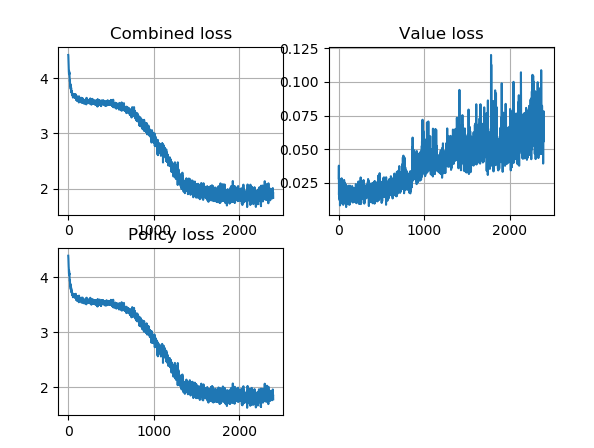
\includegraphics[width=.9\textwidth]{figures/loss-2400}
	\caption{Training loss rates for H2 after 2,400 training iterations.}
	\label{fig-loss-2400}
\end{figure}
